% ------------------------------------------------------------------------------
% TYPO3 Version 10.4 - What's New (English Version)
%
% @author	Michael Schams <schams.net>
% @license	Creative Commons BY-NC-SA 3.0
% @link		https://typo3.org/help/documentation/whats-new/
% @language	English
% ------------------------------------------------------------------------------

\documentclass[t]{beamer}

% suppress navigation bar
\beamertemplatenavigationsymbolsempty

\mode<presentation>
{
	\usetheme{typo3slides}
}

% global variables
\title{TYPO3 Version 10.4 - What's New}
\subtitle{Summary of the new features, changes and improvements}
\author{
	\centerline{Created by:}
	\centerline{Michael Schams}
}

\date{\today}

\begin{document}

% select TYPO3 Share font
\sharefont

% ------------------------------------------------------------------------------
% Title Page
% ------------------------------------------------------------------------------

\begingroup
	\setbeamercolor{normal text}{fg=white,bg=typo3orange}
	\setbeamercolor{title}{fg=white}
	\setbeamercolor{author}{fg=white}
	\setbeamertemplate{footline}[default]
	\begin{frame}
		\titlepage
	\end{frame}
\endgroup

% ------------------------------------------------------------------------------
% Table of Contents
% ------------------------------------------------------------------------------

\section*{TYPO3 Version 10.4 - What's New}
\begin{frame}[fragile]
	\frametitle{Chapter Overview}
	\framesubtitle{Chapter Overview}

	\tableofcontents

\end{frame}

% ------------------------------------------------------------------------------

% ------------------------------------------------------------------------------
% TYPO3 Version 10.0 - What's New (English Version)
%
% @author	Michael Schams <schams.net>
% @license	Creative Commons BY-NC-SA 3.0
% @link		http://typo3.org/download/release-notes/whats-new/
% @language	English
% ------------------------------------------------------------------------------

\section{Introduzione}
\begin{frame}[fragile]
	\frametitle{Introduzione}

	\begin{center}\huge{Introduzione}\end{center}
	\begin{center}\huge{\color{typo3darkgrey}\textbf{I fatti in breve}}\end{center}

\end{frame}

% ------------------------------------------------------------------------------
% TYPO3 Version 10.0 - The Facts

\begin{frame}[fragile]
	\frametitle{Introduzione}
	\framesubtitle{TYPO3 Versione 10.0 - I fatti in breve}

	\begin{itemize}
		\item Data di rilascio: 23 Luglio 2019
		\item Tipo di rilascio: Sprint Release
		\item Tempi di sviluppo: circa 6 mesi
	\end{itemize}

	\begin{figure}
		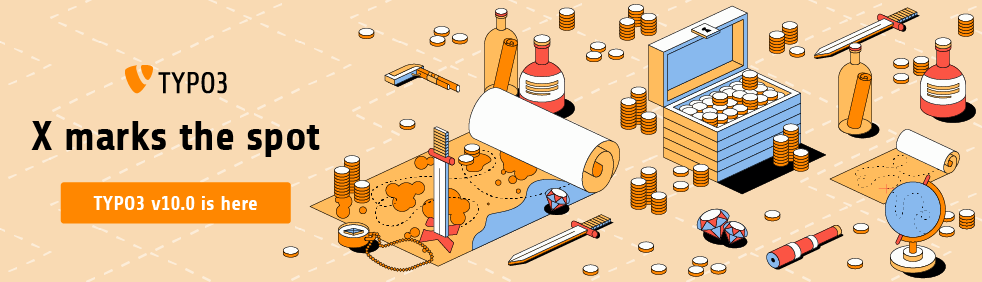
\includegraphics[width=0.95\linewidth]{Introduction/typo3-v10-0-banner.png}
	\end{figure}

\end{frame}

% ------------------------------------------------------------------------------
% TYPO3 Version 10.0 - Executive Summary

\begin{frame}[fragile]
	\frametitle{Introduzione}
	\framesubtitle{Rapporto di sintesi}

	\small
		TYPO3 versione 10.0 è la prima sprint release per arrivare alla versione LTS
		(long-term support) nel 2020.

		\vspace{0.2cm}

		Poichè l'obiettivo principale della versione 10.0 è centrato sulle attività di pulizia, non
		sorprende che in questa versione siano state introdotte numerose modifiche importanti.

		\vspace{0.2cm}

		Questo approccio ci permette di introdurre nuove librerie, concetti moderni e
		semplificare le API in una fase iniziale dello sviluppo per garantire che TYPO3
		rimanga uno dei migliori sistemi  di gestione dei contenuti aziendali sul mercato.

		\vspace{0.2cm}

		Sono state inoltre formate una serie di interessanti
		\href{https://typo3.org/community/teams/typo3-development/initiatives/}{iniziative}
		per apportare miglioramenti a lungo termine in aree specifiche di TYPO3.
	\normalsize

\end{frame}

% ------------------------------------------------------------------------------
% System Requirements

\begin{frame}[fragile]
	\frametitle{Introduzione}
	\framesubtitle{Requisiti di sistema}

	\begin{itemize}
		\item PHP versione 7.2 o 7.3
		\item Impostazioni PHP:

			\begin{itemize}
				\item \texttt{memory\_limit} >= 256M
				\item \texttt{max\_execution\_time} >= 240s
				\item \texttt{max\_input\_vars} >= 1500
				\item l'opzione di compilazione \texttt{-}\texttt{-disable-ipv6} \underline{non} deve essere usata
			\end{itemize}

		\item La maggior parte dei database supportati da \textbf{Doctrine DBAL} funzionano anche con TYPO3.
			I DB verificati sono ad esempio:
	\end{itemize}

	\begin{figure}
		
\includegraphics[width=0.80\linewidth]{Introduction/logo-databases.png}
	\end{figure}

\end{frame}

% ------------------------------------------------------------------------------
% Development, Release and Maintenance Timeline

\begin{frame}[fragile]
	\frametitle{Introduzione}
	\framesubtitle{Sviluppo, tempi di rilascio e mantenimento}

	\textbf{TYPO3 v10}

	\begin{figure}
		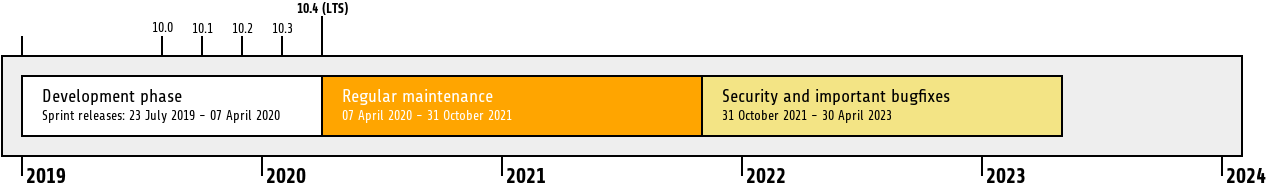
\includegraphics[width=1\linewidth]{Introduction/typo3-v10-lifecycle.png}
	\end{figure}

	\textbf{Extended Support}\newline
	\smaller
		La \href{https://typo3.com}{TYPO3 GmbH} offre ulteriori opzioni di supporto
		per TYPO3 v10 LTS anche dopo il 30 Aprile 2023, per ulteriori due anni.
	\normalsize

\end{frame}

% ------------------------------------------------------------------------------
% TYPO3 v10 Roadmap

\begin{frame}[fragile]
	\frametitle{Introduzione}
	\framesubtitle{TYPO3 v10 Roadmap}

	Date di rilascio e loro obiettivi principali:

	\begin{itemize}

		\item
			\begingroup
				\color{typo3orange}
				v10.0 \tabto{1.1cm}23/Lug/2019\tabto{3.4cm}Preparare la strada per nuovi concetti e API entusiasmanti
			\endgroup
		\item v10.1 \tabto{1.1cm}01/Ott/2019\tabto{3.4cm}Miglioramenti nel routing e nel gestore di sito v2
		\item v10.2 \tabto{1.1cm}03/Dic/2019\tabto{3.4cm}Miglioramenti al motore di rendering Fluid
		\item v10.3 \tabto{1.1cm}04/Feb/2020\tabto{3.4cm}Conferma della funzionalità
		\item v10.4 \tabto{1.1cm}07/Apr/2020\tabto{3.4cm}Rilascio LTS (Long-term Support)

	\end{itemize}

	\smaller
		\url{https://typo3.org/article/typo3-v10-roadmap/}\newline
		\url{https://typo3.org/article/typo3-v10-safe-and-sound/}
	\normalsize

\end{frame}

% ------------------------------------------------------------------------------
% Installation

\begin{frame}[fragile]
	\frametitle{Introduzione}
	\framesubtitle{Installazione}

	\begin{itemize}
		\item Procedura ufficiale, \textit{classica}, di installazione in Linux/Mac OS X\newline
			(Directory Root ad esempio \texttt{/var/www/site/htdocs}):
		\begin{lstlisting}
$ cd /var/www/site
$ wget --content-disposition get.typo3.org/10.0
$ tar xzf typo3_src-10.0.0.tar.gz
$ cd htdocs
$ ln -s ../typo3_src-10.0.0 typo3_src
$ ln -s typo3_src/index.php
$ ln -s typo3_src/typo3
$ touch FIRST_INSTALL
		\end{lstlisting}

		\item Link simbolici in Microsoft Windows:

			\begin{itemize}
				\item Usa \texttt{junction} in Windows XP/2000
				\item Usa \texttt{mklink} in Windows Vista e Windows 7 e superiori
			\end{itemize}

	\end{itemize}
\end{frame}

% ------------------------------------------------------------------------------
% Installation using composer

\begin{frame}[fragile]
	\frametitle{Installazione e aggiornamento}
	\framesubtitle{Installazione con \texttt{composer}}

	\begin{itemize}
		\item Installazione con \textit{composer} in Linux, Mac OS X e Windows 10:

			\begin{lstlisting}
$ cd /var/www/site/
$ composer create-project typo3/cms-base-distribution typo3v10 ^10
			\end{lstlisting}

		\item In alternativa, create il vostro file \texttt{composer.json} ed eseguite:

			\begin{lstlisting}
$ composer install
			\end{lstlisting}

			Maggiori informazioni e un esempio di file \texttt{composer.json} sono disponibili su:\newline
			\smaller
				\href{https://composer.typo3.org}{https://composer.typo3.org}
			\normalsize

	\end{itemize}
\end{frame}

% ------------------------------------------------------------------------------

% ------------------------------------------------------------------------------
% TYPO3 Version 10.2 - What's New (German Version)
%
% @license	Creative Commons BY-NC-SA 3.0
% @link		http://typo3.org/download/release-notes/whats-new/
% @language	German
% ------------------------------------------------------------------------------

\section{Backend User Interface}
\begin{frame}[fragile]
	\frametitle{Backend User Interface}

	\begin{center}\huge{Kapitel 1:}\end{center}
	\begin{center}\huge{\color{typo3darkgrey}\textbf{Backend User Interface}}\end{center}

\end{frame}

% ------------------------------------------------------------------------------
% Feature | 89458 | Show link to online docs in extension manager

\begin{frame}[fragile]
	\frametitle{Backend User Interface}
	\framesubtitle{Extension Manager}

	Der Extension Manager zeigt nun Links zur Extension-Dokumentation an.

	\begin{figure}
		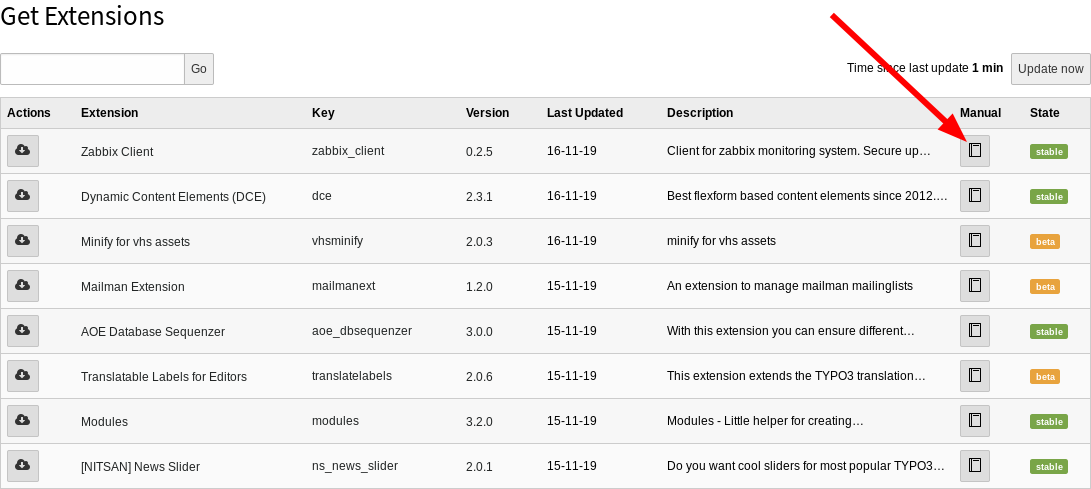
\includegraphics[width=0.90\linewidth]{ChangesForIntegrators/89458-ShowLinkToOnlineDocsInExtensionManager.png}
	\end{figure}

\end{frame}

% ------------------------------------------------------------------------------
% Feature | 86818 | Reintroduce keyboard accessible version of the pagetree

\begin{frame}[fragile]
	\frametitle{Backend User Interface}
	\framesubtitle{Zugänglichkeit Seitenbaum}

	Backend-Benutzer können nun mit ihrer Tastatur durch den Seitenbaum navigieren.
	Zum Beispiel mit den Pfeiltasten, "Home", "End", "Enter", "Space", usw.
	\newline
	Dies entspricht den Best Practices, wie sie in
	\href{https://www.w3.org/TR/wai-aria-practices-1.1/#keyboard-interaction-22}{WAI-ARIA Authoring Practices 1.1}
	vom W3C beschrieben wurden.

	\begin{figure}
		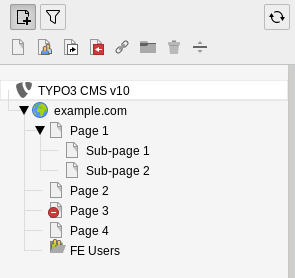
\includegraphics[width=0.30\linewidth]{BackendUserInterface/86818-PagetreeAccessibility.png}
	\end{figure}

\end{frame}

% ------------------------------------------------------------------------------

% ------------------------------------------------------------------------------
% TYPO3 Version 10.2 - What's New (English Version)
%
% @author	Michael Schams <schams.net>
% @license	Creative Commons BY-NC-SA 3.0
% @link		http://typo3.org/download/release-notes/whats-new/
% @language	English
% ------------------------------------------------------------------------------

\section{Changes for Integrators}
\begin{frame}[fragile]
	\frametitle{Changes for Integrators}

	\begin{center}\huge{Chapter 2:}\end{center}
	\begin{center}\huge{\color{typo3darkgrey}\textbf{Changes for Integrators}}\end{center}

\end{frame}

% ------------------------------------------------------------------------------
% Feature | 85592 | Add site title configuration to sites module

\begin{frame}[fragile]
	\frametitle{Changes for Integrators}
	\framesubtitle{Site Configuration (1)}

	\begin{itemize}

		\item The site title can now be configured in
			\textbf{SITE CONFIGURATION} $\rightarrow$ \textbf{Sites}.
		\item This lets integrators specify different site titles per language.
		\item The field in the template record is obsolete and has been marked as \textbf{deprecated}.
		\item The field \texttt{sys\_template.sitetitle} (database and TCA) will be removed in TYPO3 v11.
		\item The site title is used for the page title as well as for
			future \texttt{schema.org} integrations.
	\end{itemize}

\end{frame}

% ------------------------------------------------------------------------------
% Feature | 89398 | Support for environment variables in imports in site configurations

\begin{frame}[fragile]
	\frametitle{Changes for Integrators}
	\framesubtitle{Site Configuration (2)}

	% decrease font size for code listing
	\lstset{basicstyle=\tiny\ttfamily}

	\begin{itemize}

		\item It is now possible to use environment variables in imports of site configuration YAML files:
\begin{lstlisting}
imports:
  -
    resource: 'Env_%env("foo")%.yaml'
\end{lstlisting}

	\end{itemize}

\end{frame}

% ------------------------------------------------------------------------------
% Feature | 88102 | Frontend Login Form Via Fluid And Extbase

\begin{frame}[fragile]
	\frametitle{Changes for Integrators}
	\framesubtitle{Frontend Login (1)}

	\begin{itemize}

		\item TYPO3 v10.2 now includes an Extbase-version of the frontend login functionality.
		\item This solution has a few advantages:

			\begin{itemize}
				\item Modify the templates more easily.
				\item Send out HTML-based password recovery emails.
				\item Adjust and modify validators to enforce password restrictions.
			\end{itemize}

		\item The new Extbase plugin is available out-of-the-box for new installations.
		\item Existing TYPO3 instances will continue to use the old templates.
		\item Integrators can switch between the "old" and the "new" plugin by using a feature toggle.

	\end{itemize}

\end{frame}

% ------------------------------------------------------------------------------
% Feature | 88110 | Felogin extbase password recovery

\begin{frame}[fragile]
	\frametitle{Changes for Integrators}
	\framesubtitle{Frontend Login (2)}

	\begin{itemize}

		\item A password recovery form has been added as part of the Extbase plugin.
		\item Users can request a password change and will receive an email with a link which redirects them to the form.
		\item Default password validation rules:

			\begin{itemize}
				\item \texttt{NotEmptyValidator} - passwords cannot be empty.
				\item \texttt{StringLengthValidator} - passwords must have a minimum length.
			\end{itemize}

	\end{itemize}

\end{frame}

% ------------------------------------------------------------------------------
% Feature | 88110 | Felogin extbase password recovery

\begin{frame}[fragile]
	\frametitle{Changes for Integrators}
	\framesubtitle{Frontend Login (3)}

	% decrease font size for code listing
	\lstset{basicstyle=\tiny\ttfamily}

	\begin{itemize}
		\item These validation rules can be customized.
		\item For example:
\begin{lstlisting}
plugin.tx_felogin_login {
  settings {
    passwordValidators {
      10 = TYPO3\CMS\Extbase\Validation\Validator\AlphanumericValidator
      20 {
        className = TYPO3\CMS\Extbase\Validation\Validator\StringLengthValidator
        options {
          minimum = 12
          maximum = 32
        }
      }
      30 = \Vendor\MyExtension\Validation\Validator\MyCustomPasswordPolicyValidator
    }
  }
}
\end{lstlisting}

	\end{itemize}

\end{frame}

% ------------------------------------------------------------------------------
% Feature | 89526 | FeatureFlag: betaTranslationServer

\begin{frame}[fragile]
	\frametitle{Changes for Integrators}
	\framesubtitle{Localization Management Platform}

	\begin{itemize}

		\item \href{https://crowdin.com/}{crowdin} aims to replace the existing
			\href{https://translation.typo3.org/}{Pootle}
			solution as a localization/translation management platform.

		\item A feature toggle has been added in TYPO3 v10.2 that uses crowdin.com
			as the source for translations if enabled.

		\item Please note: this is in \textbf{beta status}.

		\item Read more about the
			\href{https://typo3.org/community/teams/typo3-development/initiatives/localization-with-crowdin/}{initiative}.

	\end{itemize}

	\begin{figure}
		
\includegraphics[width=0.50\linewidth]{ChangesForIntegrators/crowdin-logo.png}
	\end{figure}

\end{frame}

% ------------------------------------------------------------------------------
% Feature | 89171 | Added possibility to have multiple sitemaps

\begin{frame}[fragile]
	\frametitle{Changes for Integrators}
	\framesubtitle{Multiple Sitemaps}

	% decrease font size for code listing
	\lstset{basicstyle=\tiny\ttfamily}

	\begin{itemize}

		\item It is now possible to configure multiple sitemaps.
		\item Syntax:
\begin{lstlisting}
plugin.tx_seo {
  config {
    <sitemapType> {
      sitemaps {
        <unique key> {
          provider = TYPO3\CMS\Seo\XmlSitemap\RecordsXmlSitemapDataProvider
          config {
            ...
          }
        }
      }
    }
  }
}
\end{lstlisting}

	\end{itemize}

\end{frame}

% ------------------------------------------------------------------------------
% Feature | 86759 | Support nomodule attribute for JavaScript includes

\begin{frame}[fragile]
	\frametitle{Changes for Integrators}
	\framesubtitle{HTML5 attribute \texttt{nomodule}}

	% decrease font size for code listing
	\lstset{basicstyle=\tiny\ttfamily}

	\begin{itemize}
		\item The HTML5 attribute \texttt{nomodule} is now supported when including JavaScript files in TypoScript.
\begin{lstlisting}
page.includeJSFooter.file = path/to/classic-file.js
page.includeJSFooter.file.nomodule = 1
\end{lstlisting}

		\item This attribute prevents a script from being executed in browsers that support module scripts.

		\item Read more about the standard in the
			\href{https://html.spec.whatwg.org/multipage/scripting.html#attr-script-nomodule}{specification}
			and about the concept of
			\href{https://hacks.mozilla.org/2015/08/es6-in-depth-modules/}{modules}.

	\end{itemize}

% <script type="module" src="path/to/file.js"></script>
% <script nomodule src="path/to/file/classic-file.js"></script>

\end{frame}

% ------------------------------------------------------------------------------
% Feature | 87798 | Provide a way to sort form lists in ext:form

\begin{frame}[fragile]
	\frametitle{Changes for Integrators}
	\framesubtitle{Sorting of Forms}

	% decrease font size for code listing
	\lstset{basicstyle=\tiny\ttfamily}

	\begin{itemize}
		\item Forms can now be sorted in either ascending or descending order.
		\item Two new settings were introduced: \texttt{sortByKeys} and \texttt{sortAscending}.
		\item Forms are initially sorted by their name and their file UID (ascending).
		\item To change the sorting, the following configuration needs to be added in the YAML configuration file:
\begin{lstlisting}
TYPO3:
  CMS:
    Form:
      persistenceManager:
        sortByKeys: ['name', 'fileUid']
        sortAscending: true
\end{lstlisting}

	\end{itemize}

\end{frame}

% ------------------------------------------------------------------------------
% Feature | 86918 | Add additional configuration for external link types in Linkvalidator

\begin{frame}[fragile]
	\frametitle{Changes for Integrators}
	\framesubtitle{Link Validator (1)}

	% decrease font size for code listing
	\lstset{basicstyle=\tiny\ttfamily}

	\begin{itemize}
		\item The Link Validator now supports additional configuration for external links.
		\item Values for \texttt{httpAgentUrl} and \texttt{httpAgentEmail} should be provided.
		\item Settings \texttt{headers}, \texttt{method} and \texttt{range} are advanced settings.
\begin{lstlisting}
mod.linkvalidator {
  linktypesConfig {
    external {
      httpAgentName = ...
      httpAgentUrl = ...
      httpAgentEmail = ...
      headers {
      }
      method = HEAD
      range = 0-4048
    }
  }
}
\end{lstlisting}

	\end{itemize}

\end{frame}

% ------------------------------------------------------------------------------
% Feature | 84990 | Add event for checking external links in RTE

\begin{frame}[fragile]
	\frametitle{Changes for Integrators}
	\framesubtitle{Link Validator (2)}

	\begin{itemize}
		\item Link Validator now marks broken \textbf{external} links in the RTE too.
		\item This feature was only available for internal links.
		\item It is recommended to run the Link Validator as a Scheduler task to regularly crawl for broken links.
	\end{itemize}

\end{frame}

% ------------------------------------------------------------------------------

% ------------------------------------------------------------------------------
% TYPO3 Version 10.2 - What's New (Serbian Version)
%
% @license	Creative Commons BY-NC-SA 3.0
% @link		http://typo3.org/download/release-notes/whats-new/
% @language	Serbian
% ------------------------------------------------------------------------------

\section{Izmene za programere}
\begin{frame}[fragile]
	\frametitle{Izmene za programere}

	\begin{center}\huge{Poglavlje 3:}\end{center}
	\begin{center}\huge{\color{typo3darkgrey}\textbf{Izmene za programere}}\end{center}

\end{frame}

% ------------------------------------------------------------------------------
% Feature | 88950 | Add storeSession argument to Widget ViewHelpers

\begin{frame}[fragile]
	\frametitle{Izmene za programere}
	\framesubtitle{Widget ViewHelper-i}

	% decrease font size for code listing
	\lstset{basicstyle=\smaller\ttfamily}

	\begin{itemize}
		\item Widget ViewHelper-i u odredjenim situacijama postavljaju session cookie na korisničkom interfejsu.
		\item Pošto ovo nije poželjno u svim situacijama (na primer zbog GDPR), sada može da se kontroliše.
		\item Boolean promenljiva \texttt{storeSession} je dodata da omogući programerima da omoguće/onemoguće
		 	ovu funkcionalnost.
\begin{lstlisting}
<f:widget.autocomplete
  for="name"
  objects="{posts}"
  searchProperty="author"
  storeSession="false" />
\end{lstlisting}

	\end{itemize}

\end{frame}

% ------------------------------------------------------------------------------
% Feature | 89577 | New PSR-14 based events for File Abstraction Layer
% Deprecation | 89577 | FAL SignalSlot handling migrated to PSR-14 events

\begin{frame}[fragile]
	\frametitle{Izmene za programere}
	\framesubtitle{PSR-14 dogadjaji u FAL}

	% decrease font size for code listing
	\lstset{basicstyle=\tiny\ttfamily}

	\begin{itemize}
		\item U File Abstraction Layer (FAL) dodato je oko 40 novih dogadjaja zasnovanih na
			\href{https://www.php-fig.org/psr/psr-14/}{PSR-14}.
		\item Oni zamenjuju postojeće Extbase signale/slotove.
		\item Korišćenje signala i dalje radi (bez poruke o zastarelosti!).
			Medjutim, signali iz FAL-a će najverovatnije biti uklonjeni u TYPO3 v11.
		\item Autori proširenja se savetuju da migriraju kod i koriste dogadjaje.
		\item Pogledajte novie PHP klase da saznate više o PSR-14.
	\end{itemize}

\end{frame}


% ------------------------------------------------------------------------------
% Deprecation | 89733 | Signal Slots in Core Extension migrated to PSR-14 events

\begin{frame}[fragile]
	\frametitle{Izmene za programere}
	\framesubtitle{PSR-14 dogadjaji u jezgru TYPO3}

	\begin{itemize}
		\item Veliki broj novih dogadjaja zasnovanih na PSR-14 zamenuje signale/slotove u jezgru TYPO3:
			\newline

			\begin{itemize}\tiny
				\item \texttt{TYPO3\textbackslash
					CMS\textbackslash
					Core\textbackslash
					Imaging\textbackslash
					Event\textbackslash
					ModifyIconForResourcePropertiesEvent}
					\newline
				\item \texttt{TYPO3\textbackslash
					CMS\textbackslash
					Core\textbackslash
					DataHandling\textbackslash
					Event\textbackslash
					IsTableExcludedFromReferenceIndexEvent}
					\newline
				\item \texttt{TYPO3\textbackslash
					CMS\textbackslash
					Core\textbackslash
					DataHandling\textbackslash
					Event\textbackslash
					AppendLinkHandlerElementsEvent}
					\newline
				\item \texttt{TYPO3\textbackslash
					CMS\textbackslash
					Core\textbackslash
					Configuration\textbackslash
					Event\textbackslash
					AfterTcaCompilationEvent}
					\newline
				\item \texttt{TYPO3\textbackslash
					CMS\textbackslash
					Core\textbackslash
					Database\textbackslash
					Event\textbackslash
					AlterTableDefinitionStatementsEvent}
					\newline
				\item \texttt{TYPO3\textbackslash
					CMS\textbackslash
					Core\textbackslash
					Tree\textbackslash
					Event\textbackslash
					ModifyTreeDataEvent}
					\newline
				\item \texttt{TYPO3\textbackslash
					CMS\textbackslash
					Backend\textbackslash
					Backend\textbackslash
					Event\textbackslash
					SystemInformationToolbarCollectorEvent}
					\newline
			\end{itemize}

	\end{itemize}

\end{frame}

% ------------------------------------------------------------------------------
% Deprecation | 89718 | Legacy PageTSconfig parsing lowlevel API

\begin{frame}[fragile]
	\frametitle{Izmene za programere}
	\framesubtitle{Prepared Statements}

	% decrease font size for code listing
	\lstset{basicstyle=\tiny\ttfamily}

	\begin{itemize}
		\item Dodate su dve nove PHP klase za čitanje i parsiranje PageTSconfig:
			\begin{itemize}\smaller
				\item \texttt{TYPO3\textbackslash
					CMS\textbackslash
					Core\textbackslash
					Configuration\textbackslash
					Loader\textbackslash
					PageTsConfigLoader}
				\item \texttt{TYPO3\textbackslash
					CMS\textbackslash
					Core\textbackslash
					Configuration\textbackslash
					Parser\textbackslash
					PageTsConfigParser}
			\end{itemize}

		\item Na primer:
\begin{lstlisting}
// Fetch all available PageTS of a page/rootline:
$loader = GeneralUtility::makeInstance(PageTsConfigLoader::class);
$tsConfigString = $loader->load($rootLine);

// Parse the string and apply conditions:
$parser = GeneralUtility::makeInstance(
  PageTsConfigParser::class, $typoScriptParser, $hashCache
);

$pagesTSconfig = $parser->parse($tsConfigString, $conditionMatcher);
\end{lstlisting}

	\end{itemize}

\end{frame}

% ------------------------------------------------------------------------------
% Important | 87518 | Use prepared statements for pdo_mysql per default

\begin{frame}[fragile]
	\frametitle{Izmene za programere}
	\framesubtitle{Prepared Statements}

	% decrease font size for code listing
	\lstset{basicstyle=\tiny\ttfamily}

	\begin{itemize}
		\item Po podrazumevanim podešavanjima \texttt{pdo\_mysql} drajver koristi prepared statements.
		\item U TYPO3 < v10.2 korišćene su \textit{emulirane prepared statements}.
			Ovo znači da su sve vrednosti upita koje su vraćene bile tekstualnog tipa.
		\item Ovo ponašanje je promenjeno i prepared statements sada vraćaju nativne tipove podataka.
		\item Na primer: vrednosti za kolonu koja je definisana kao celobrojna se vraćaju u PHP kao \texttt{int}.
		\item Ova funkcionalnost može da se isključi u podešavanjima konekcije sa bazom podataka
			u opciji \texttt{PDO::ATTR\_EMULATE\_PREPARES}.

	\end{itemize}

\end{frame}

% ------------------------------------------------------------------------------
% Feature | 86967 | Allow fetching uid of a LazyLoadingProxy without loading the object first

\begin{frame}[fragile]
	\frametitle{Izmene za programere}
	\framesubtitle{Lazy Loading Proxy}

	% decrease font size for code listing
	\lstset{basicstyle=\tiny\ttfamily}

	\begin{itemize}
		\item Metod \texttt{getUid()} je dodat klasi\newline
			\texttt{TYPO3\textbackslash
				CMS\textbackslash
				Extbase\textbackslash
				Persistence\textbackslash
				Generic\textbackslash
				LazyLoadingProxy}.
		\item Ovo omogućava programerima da dodju do UID-a objekta koji je iza proksija,
			bez potrebe da se objekat dovlači iz baze podataka.

	\end{itemize}

\end{frame}

% ------------------------------------------------------------------------------
% Feature | 87380 | Introduce SiteLanguageAwareInterface to denote site language awareness

\begin{frame}[fragile]
	\frametitle{Izmene za programere}
	\framesubtitle{Označavanje jezika sajta}

	% decrease font size for code listing
	\lstset{basicstyle=\tiny\ttfamily}

% SiteLanguageAwareInterface with the methods setSiteLanguage(Entity\SiteLanguage $siteLanguage) and getSiteLanguage() has been introduced.
% The interface can be used to denote a class as aware of the site language.

	\begin{itemize}
		\item \texttt{SiteLanguageAwareInterface} je dodat.
		\item Interfejs se može koristiti da označi da je klasa svesna jezika sajta.
		\item Aspekti rutiranja, koji uzimaju u obzir jezik sajta,
			sada koriste i \texttt{SiteLanguageAwareInterface}
			uz \texttt{SiteLanguageAwareTrait}.
	\end{itemize}

\end{frame}

% ------------------------------------------------------------------------------
% Important | 89645 | Removed systemLog options

\begin{frame}[fragile]
	\frametitle{Izmene za programere}
	\framesubtitle{System Log API}

	% decrease font size for code listing
	\lstset{basicstyle=\tiny\ttfamily}

	\begin{itemize}
		\item Sledeće opcije su uklonjene iz podrazumevane konfiguracije TYPO3:

			\begin{itemize}\smaller
				\item \texttt{\$GLOBALS['TYPO3\_CONF\_VARS']['SYS']['systemLog']}
				\item \texttt{\$GLOBALS['TYPO3\_CONF\_VARS']['SYS']['systemLogLevel']}
			\end{itemize}\normalsize

		\item Autori proširenja se savetuju da koriste Logging API i uklone systemLog opcije.
	\end{itemize}

\end{frame}

% ------------------------------------------------------------------------------
% Feature | 89603 | Introduce native pagination for lists

\begin{frame}[fragile]
	\frametitle{Izmene za programere}
	\framesubtitle{Podrazumevana paginacija lista}

	% decrease font size for code listing
	\lstset{basicstyle=\tiny\ttfamily}

	\begin{itemize}
		\item Dodata je podrazumevana podrška za paginaciju lista kao što su nizovi i Extbase QueryResults.
		\item \texttt{PaginatorInterface} definiše osnovni skup metoda.
		\item \texttt{AbstractPaginator} klasa sadrži osnovnu logiku za paginaciju.
		\item Ovo omogućava programerima da naprave paginatore po svojoj potrebi.
\begin{lstlisting}
use TYPO3\CMS\Core\Pagination\ArrayPaginator;

$items = ['apple', 'banana', 'strawberry', 'raspberry', 'ananas'];
$currentPageNumber = 3;
$itemsPerPage = 2;

$paginator = new ArrayPaginator($itemsToBePaginated, $currentPageNumber, $itemsPerPage);
$paginator->getNumberOfPages(); // returns 3
$paginator->getCurrentPageNumber(); // returns 3
$paginator->getKeyOfFirstPaginatedItem(); // returns 5
$paginator->getKeyOfLastPaginatedItem(); // returns 5
\end{lstlisting}

	\end{itemize}

\end{frame}

% ------------------------------------------------------------------------------
% Deprecation | 89579 | ServiceChains require an array for excluded Service keys

\begin{frame}[fragile]
	\frametitle{Izmene za programere}
	\framesubtitle{API za servise}

	\begin{itemize}
		\item Argument \texttt{\$excludeServiceKeys} se koristi da se preskoči odredjeni servis kada se koristi lanac servisa.
		\item U TYPO3 v10.2 argument je promenjen iz liste razdvojene zarezom u niz.
		\item Ova izmena utiče na API za servise kod sledećih komponenti:

			\begin{itemize}
				\item \texttt{GeneralUtility::makeInstanceService()}
				\item \texttt{ExtensionManagementUtility::findService()}
			\end{itemize}

		\item Prosledjivanje liste razdvojene zarezom i dalje radi, ali je označeno kao \textbf{zastarelo}.

	\end{itemize}

\end{frame}

% ------------------------------------------------------------------------------

% ------------------------------------------------------------------------------
% TYPO3 Version 10.3 - What's New (Dutch Version)
%
% @license	Creative Commons BY-NC-SA 3.0
% @link		https://typo3.org/help/documentation/whats-new/
% @language	Dutch
% ------------------------------------------------------------------------------

\section{Verouderde/verwijderde functies}
\begin{frame}[fragile]
	\frametitle{Verouderde/verwijderde functies}

	\begin{center}\huge{Hoofdstuk 4:}\end{center}
	\begin{center}\huge{\color{typo3darkgrey}\textbf{Verouderde/verwijderde functies}}\end{center}

\end{frame}

% ------------------------------------------------------------------------------
% Deprecation | 89463 | Deprecate switchable controller actions

\begin{frame}[fragile]
	\frametitle{Verouderde/verwijderde functies}
	\framesubtitle{Switchable Controller Actions}

	\begin{itemize}
		\item "Switchable Controller Actions" (SCA) zijn als \textbf{verouderd} aangemerkt.
		\item SCA kunnen de toegestane set van controllers en actions overschrijven via TypoScript of Flexforms.
		\item Dezelfde plug-in gebruiken voor veel verschillende functionaliteiten gaat in tegen het idee dat een plug-in een bepaald doel heeft.
		\item Plug-ins die SCA gebruiken moeten opgedeeld worden in meerdere plug-ins.
	\end{itemize}

\end{frame}

% ------------------------------------------------------------------------------
% Deprecation | 90007 | Global constants TYPO3_version and TYPO3_branch

\begin{frame}[fragile]
	\frametitle{Verouderde/verwijderde functies}
	\framesubtitle{Globale constanten}

	% decrease font size for code listing
	\lstset{basicstyle=\smaller\ttfamily}

	\begin{itemize}
		\item De volgende twee globale constanten zijn als \textbf{verouderd} aangemerkt:

			\begin{itemize}
				\item \texttt{TYPO3\_version}
				\item \texttt{TYPO3\_branch}
			\end{itemize}

		\item De volgende nieuwe PHP klasse kan hiervoor gebruikt worden:\newline
			\small
				\texttt{TYPO3\textbackslash
					CMS\textbackslash
					Core\textbackslash
					Information\textbackslash
					Typo3Version}\normalsize

	\end{itemize}

\end{frame}

% ------------------------------------------------------------------------------
% Deprecation | 89673 | Deprecate Extbases WebRequest and WebResponse

\begin{frame}[fragile]
	\frametitle{Verouderde/verwijderde functies}
	\framesubtitle{Extbase: \texttt{WebRequest}/\texttt{WebResponse}}

	\begin{itemize}
		\item De volgende twee Extbase klassen zijn als \textbf{verouderd} aangemerkt:
			\begin{itemize}
				\item \texttt{TYPO3\textbackslash
					CMS\textbackslash
					Extbase\textbackslash
					Mvc\textbackslash
					Web\textbackslash
					Request}
				\item \texttt{TYPO3\textbackslash
					CMS\textbackslash
					Extbase\textbackslash
					Mvc\textbackslash
					Web\textbackslash
					Response}
			\end{itemize}

	\end{itemize}

\end{frame}

% ------------------------------------------------------------------------------
% Deprecation | 90258 | Simplified RTE Parser API

\begin{frame}[fragile]
	\frametitle{Verouderde/verwijderde functies}
	\framesubtitle{Versimpelde RTE Parser API}

	\begin{itemize}
		\item De PHP klasse \texttt{RteHtmlParser} heeft een versimpelde API.
		\item Een gevolg is dat deze twee methodes als \textbf{verouderd} zijn aangemerkt:

			\begin{itemize}
				\item \texttt{TYPO3\textbackslash
					CMS\textbackslash
					Core\textbackslash
					Html\textbackslash
					RteHtmlParser->init()}
				\item \texttt{TYPO3\textbackslash
					CMS\textbackslash
					Core\textbackslash
					Html\textbackslash
					RteHtmlParser->RTE\_transform()}
			\end{itemize}

	\end{itemize}

\end{frame}

% ------------------------------------------------------------------------------
% Deprecation | 89139 | Console Commands configuration migrated to Symfony service tags

\begin{frame}[fragile]
	\frametitle{Verouderde/verwijderde functies}
	\framesubtitle{Configuratie van console commando's}

	\begin{itemize}
		\item Aangezien de configuratie van console commando's omgezet is naar Symfony service tags,
			is het bestand met de configuratie \texttt{Configuration/Commands.php} als
			\textbf{verouderd} aangemerkt.
		\item Gebruik de service tag voor het injecteren van afhankelijkheden \texttt{console.command} hiervoor.

	\end{itemize}

\end{frame}

% ------------------------------------------------------------------------------
% Important | 89672 | transOrigPointerField is not longer allowed to be excluded

\begin{frame}[fragile]
	\frametitle{Verouderde/verwijderde functies}
	\framesubtitle{TCA: \texttt{transOrigPointerField}}

	\begin{itemize}
		\item Het uitzonderen van deze TCA-optie zorgde voor inconsistente data in de databse onder bepaalde omstandigheden:
			\small
				\texttt{\$GLOBALS['TCA'][\$table]['ctrl']['transOrigPointerField']}
			\normalsize

		\item Daarom kan de optie niet meer uitgezonderd worden.
		\item Een migratie-assistent verwijdert de optie uit de TCA en voegt een verouderingsmelding
			toe aan de verouderingslog als code bijgewerkt moet worden.
	\end{itemize}

\end{frame}

% ------------------------------------------------------------------------------
% Deprecation | 90421 | DocumentTemplate

\begin{frame}[fragile]
	\frametitle{Verouderde/verwijderde functies}
	\framesubtitle{DocumentTemplate}

	% decrease font size for code listing
	\lstset{basicstyle=\tiny\ttfamily}

	\begin{itemize}
		\item De volgende klasse is als \textbf{verouderd} aangemerkt:

			\begin{itemize}
				\item \texttt{TYPO3\textbackslash
					CMS\textbackslash
					Backend\textbackslash
					Template\textbackslash
					DocumentTemplate}
			\end{itemize}

		\item Het werd gebruikt als basis voor de weergave van backend modules of HTML-uitvoer in de TYPO3 backend.
		\item Sinds TYPO3 v7 moet de nieuwe API via ModuleTemplate gebruikt worden hiervoor.

\vspace{-0.4cm}
\begin{lstlisting}
use TYPO3\CMS\Backend\Template\ModuleTemplate;
...
$moduleTemplate = GeneralUtility::makeInstance(ModuleTemplate::class);
$content = $this->getHtmlContentFromMyModule();
$moduleTemplate->setTitle('My module');
$moduleTemplate->setContent($content);
return new HtmlResponse($moduleTemplate->renderContent());
\end{lstlisting}

	\end{itemize}

\end{frame}

% ------------------------------------------------------------------------------
% Deprecation | 85613 | Introduce simple way to register category fields
%
%\begin{frame}[fragile]
%	\frametitle{Verouderde/verwijderde functies}
%	\framesubtitle{CategoryRegistry API}
%
%	\begin{itemize}
%		\item The following class has been marked as \textbf{deprecated}:
%
%			\begin{itemize}
%				\item \texttt{TYPO3\textbackslash
%					CMS\textbackslash
%					Core\textbackslash
%					Category\textbackslash
%					CategoryRegistry}
%			\end{itemize}
%
%		\item The following method has been marked as \textbf{deprecated}:
%
%			\begin{itemize}
%				\item \texttt{ExtgensionManagementUtility::makeCategorizable()}
%			\end{itemize}
%
%		\item Category fields can easily by registered by adding TCA configuration.
%
%	\end{itemize}
%
%\end{frame}
%
% ------------------------------------------------------------------------------
% Deprecation | 90390 | Deprecate BrokenLinkRepository::getNumberOfBrokenLinks() in linkvalidator

\begin{frame}[fragile]
	\frametitle{Verouderde/verwijderde functies}
	\framesubtitle{LinkValidator}

	\begin{itemize}
		\item De volgende mehtode is als \textbf{verouderd} aangemerkt:
		\newline\newline
			\smaller
				\texttt{TYPO3\textbackslash
					CMS\textbackslash
					Linkvalidator\textbackslash
					Repository\textbackslash
					BrokenLinkRepository}\newline
				\texttt{->getNumberOfBrokenLinks()}\normalsize\newline

		\item Gebruik de volgende methode in dezelfde klasse hiervoor:\newline
			\small\texttt{BrokenLinkRepository::isLinkTargetBrokenLink()}\normalsize

	\end{itemize}

\end{frame}


% ------------------------------------------------------------------------------

% ------------------------------------------------------------------------------
% TYPO3 Version 10.1 - What's New (Italian Version)
%
% @license	Creative Commons BY-NC-SA 3.0
% @link		http://typo3.org/download/release-notes/whats-new/
% @language	Italian
% ------------------------------------------------------------------------------

\section{Fonti e autori}
\begin{frame}[fragile]
	\frametitle{Fonti e autori}

	\begin{center}\huge{Capitolo 6:}\end{center}
	\begin{center}\huge{\color{typo3darkgrey}\textbf{Fonti e autori}}\end{center}

\end{frame}

% ------------------------------------------------------------------------------
% Sources

\begin{frame}[fragile]
	\frametitle{Fonti e autori}
	\framesubtitle{Fonti}

	\textbf{TYPO3 News:}
		\begin{itemize}\smaller
			\item \url{https://typo3.org/project/news/}
		\end{itemize}

	\textbf{Note sui rilasci:}
		\begin{itemize}\smaller
			\item \url{https://get.typo3.org/release-notes/10.x/TYPO3_CMS_10.1.0}
			\item \href{https://docs.typo3.org/c/typo3/cms-core/master/en-us/Changelog-10.html}{TYPO3 v10 ChangeLog}
			\item \texttt{typo3/sysext/core/Documentation/Changelog/10.1/*}
		\end{itemize}

	\textbf{TYPO3 Bug-/Issuetracker:}
		\begin{itemize}\smaller
			\item \url{https://forge.typo3.org/projects/typo3cms-core}
		\end{itemize}

	\textbf{TYPO3 e Fluid Git Repositories:}
		\begin{itemize}\smaller
			\item \url{https://git.typo3.org/Packages/TYPO3.CMS.git}
			\item \url{https://github.com/TYPO3/Fluid}
		\end{itemize}

\end{frame}

% ------------------------------------------------------------------------------
% Authors

\begin{frame}[fragile]
	\frametitle{Fonti e autori}

	\vspace{-0.6cm}

	\centerline{\textbf{TYPO3 CMS What's New Team:}}

	\begin{center}
		\centerline{Paul Blondiaux, Pierrick Caillon, Andreas Fießer}
		\centerline{Richard Haeser, Jigal van Hemert, Henrietta Kucsovan, Sinisa Mitrovic,}
		\centerline{Michael Schams e Roberto Torresani}
	\end{center}

	\vspace{0.6cm}

	\smaller\begin{center}\url{https://typo3.org/help/documentation/whats-new/}\end{center}\normalsize

	\vspace{1cm}

	\smaller\begin{center}Licensed under Creative Commons BY-NC-SA 3.0\end{center}\normalsize
	\begin{figure}\vspace*{-0.4cm}
		
\includegraphics[width=1.4cm]{SourcesAndAuthors/CreativeCommons-BY-NC-SA.png}
	\end{figure}

\end{frame}

% ------------------------------------------------------------------------------


% ------------------------------------------------------------------------------
\end{document}
